\chapter{Qt Grundlagen}

\section{Grundlagen}
\textbf{Zweck:} Erstellung von User Interfaces (im speziellen für GUIs) und plattformunabhängige Anwendungen (im Bereich Desktop, Embedded und Mobile) \\
\textbf{Anwendungen:} Skype, Google Earth, Wolfram Research und viele mehr

\subsection{Qt Oberflächen}
\textbf{Qt Desktop (Qt Widgets)} \\
Qt Oberflächen basieren auf der Qt C++ Klassenbibliothek, welche für die GUI-Elemente ("Widgets") entsprechende Klassen wie QLabel, QPushButton etc. bereitstellt. Das GUI wird unter Verwendung dieser Klassenbibliothek als C++-Programm geschrieben und häufig für die Maus- und Tastaturbedienung genutzt. 
\textbf{Neben Qt Widget gibt es noch Qt-Quick (QML) und WebEngine. Der Fokus der Vorlesung liegt auf Qt Desktop.}

\textbf{Qt-Quick} \\
Qt-Quick basiert auf QML (= Qt Meta Language oder Qt Modelling Language), einer speziellen Sprache, welche das Aussehen des Programms festlegt. Verfügt über eine "Deklarative" Festlegung der Darstellung und des Verhaltens, ähnlich wie bei HTML mit Javascript. Qt-Qucik wird vielfach für mobile Applikationen mit Touchscreen Bedienung genutzt.

\textbf{WebEngine} \\
Web Engine wird für die Darstellung von Web Content mit HTML/CSS/JS verwendet. 

\subsubsection{Namenskonventionen}
\begin{itemize}
	\item "Qt" - QtCore - Hauptmodul (wird von allen Modulen genutzt); Weitere Module: QtGui, QtWdigets, QtNetwork, QtSql, QtTest
	\item "Q" - Klasse wie QObject, QApplication, QWidget, QDialog, QString
	\item "q" - globale Variable / Funktionsname wie qApp, qTranslator, qDebug(), qWarning(), qFatal()
	\item "Q\_GROSS" - Qt-Makro-Namen wie Q\_OBJECT, QCOMPARE, QEXPECT\_FAIL, QFETCH
	\item \#include <Qt-Modul- oder Klassenname" wie \#include <QtGui>, \#include <QObject> oder \#include <QString>
\end{itemize}

\section{Meta Object System} 
Dieses System bietet zusätzliche Funktionaitäten zu C++. Es unterstützt das Hollywood Prinizip mittels \textbf{Signals and Slots}. Es basiert auf QObject Klassen, Q\_QBJECT Makro und einem Meta-Object Compiler (moc). 

\subsection{QObject}
Aus der QObject Klasse wurden weitere Qt Klassen abgeleitet wie z.B. QPushBotton, QLabel, QGridLayout, QTimer und QThread. Die QObject Klasse wird zu einem header file hinzugefügt mit \textbf{\#include <QObject>}. QObjects können mit einer Parent-Child-Beziehung verknüpft werden, woraus ein ganzer QObject Tree entstehen kann. Ein Object Tree macht es einfacher eine grosse Anzahl an Dokumente, die miteinander verbunden sind, auf einen Schlag zu löschen. \\
Das Eltern-QObject wird im C'tor des Child-QObjects wie folgt angegeben:\\ 
\textbf{QLabel * child = new QLabel("0000", \&parent);}.\\
Alternativ kann setParent() verwendet werden: \\
\textbf{child->setParent(parent)}
Dies kann jedoch bezüglich der D'tor Reihenfolge problematisch sein (Siehe Prakti 2). \\
Ein Parent-Object kann beliebig viele child-Objects haben, während ein child-Object nur ein parent-Object hat. Die Löschung eines parent objects hat die automatische Löschung sämtlicher child objects zur Folge. Die Löschung eines child objects zerstört einfach die Beziehung zum parent object. 

\subsection{Meta Object Compiler (moc) \& qmake}
Der Meta Object Compiler (moc) durchsucht das header file nach Q\_OBJECT Makros und generiert ein moc\_XXX.cpp File mit dem meta-object relevanten Code erstellt. Diese Dateien müssen bei der Ausführung zur Anwendung hinzugelinkt werden. Für die Verlinkung und Ausführung von Meta Object Compiler (moc), User Interface Compiler (uic) und Resource Compiler (Rcc) wird qmake verwendet, welche diese Qt Compiler automatisch einbindet. Qmake erzeugt aus einer plattformunabhängigen Projektbeschreibung, dem Projektfile (.pro-Datei) ein plattformspezifisches 'makefile'. Diese makefile wird dann von den platformspezifischen Tools wie make dazu verwendet, um die Source-Files zu verarbeiten (compilieren, etc.). Dabei ist qmake selbst ein plattformunabhängiger make-file-Generator. \\Der Befehl lautet: \textbf{qmake <project file name>.pro} 

\begin{figure}[ht]
	\centering
	\adjustbox{width=12cm}{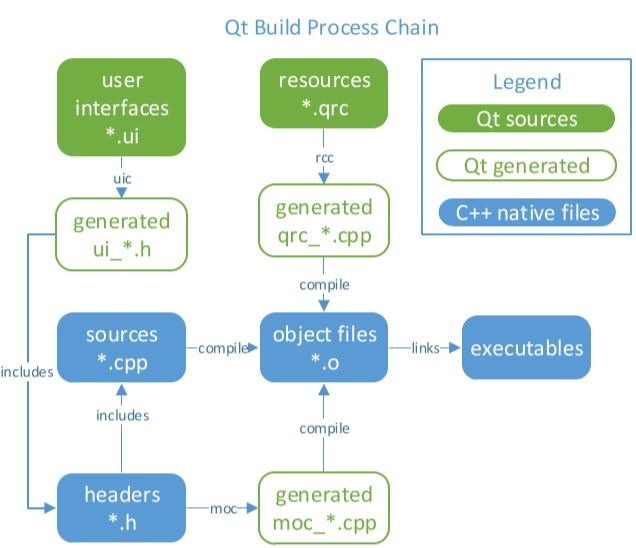
\includegraphics{Figures/qmake}}
\caption[]{Qt Build Prozessablauf}
\end{figure}

\newpage
\subsection{Projektbeschreibung (*.pro)}
\begin{multicols}{2}
\textbf{Keywords:} \\
- QT: Liste von verwendeten Qt Modulen \\
- Target: Name der Applikation (Output File) \\
- TEMPLATE: Projekt Typ: app oder lib \\
- CONFIG: z.B. CONFIG += C++14  \\
- windows/linux/macx: Plattform spezifische   Compilierungsregeln \\
- SOURCES/HEADER/FORMS: Source-, Header- oder Formdateien die dem Projekt hinzugefügt werden sollen \\
\columnbreak
\adjustbox{width=6.5cm}{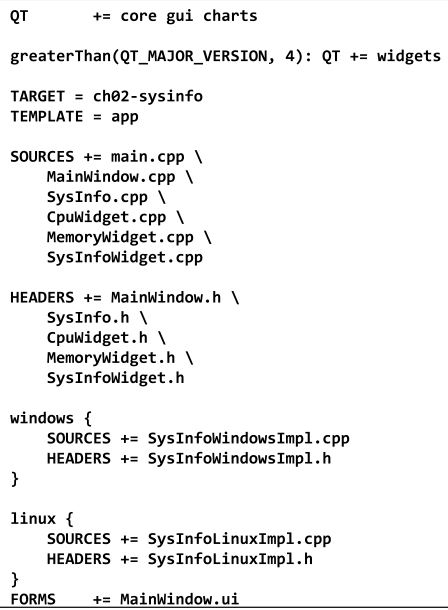
\includegraphics{Figures/keywordspro}}
\end{multicols}


\section{Qt Hallo Welt Beispiel}

\#include <QtWidgets> \\
int main(int argc, char *argv[]) \\
{	QApplication app(argc, argv); \\
	QLabel label ("Hello Qt World!"); \% Erstellen eines Textfelds mit dem Text Hello Qt World! \\
 	label.setAlignment(Qt::AlignCenter); \% Textfeld in der Mitte ausrichten \\
	label.resize(250, 150); \%Breite \& Höhe des Testfelds \\
	label.setWindowTitle("My first Qt‐Program"); \%Titel des Popup Fenster  \\
	label.show(); \%Befehl zum Anzeigen des Textfelds \\
	return app.exec(); } 

\subsection{QApplication Klasse}
Die QApplication Klasse ist pro Qt Applikation nur einmal vorhanden. Sie ist zuständig für das Event handling und weitere Qt Framework spezifische Funktionälitäten. Eine der Methoden heisst exec(). In dieser Methode verbirgt sich die while(1) Schleife.
QApplication Klasse ist zudem für die Initialisierung der Applikation mit optionalen Funktionen wie beispielsweise font() und doubleClickInterval() zuständig. 

